%\documentclass[prb,aps,nobibnotes,twocolumn,doublespace,twocolumngrid,superbib]{revtex4}
\documentclass[prb,aps,nobibnotes,superbib,preprint]{revtex4}

\usepackage{graphicx}
\usepackage{amsfonts}
\usepackage{amsmath}
\usepackage{bm}
\usepackage{alltt}
\usepackage{dcolumn} 
\usepackage{graphicx}
\makeatletter 
\makeatother

\begin{document}

\title{\textbf{An Exact Bounded Error for Multipoles}}

\author{C. J. Tymczak}
\author{Matt Challacombe}

\affiliation{Theoretical Division, Los Alamos National Laboratory, Los Alamos,NM 87545, USA}

\date{\today}

\begin{abstract}
We derive an exact error bound for the multipole approximation which is essential for the control of
errors within several important algorithms, for example the multipole tree-codes 
and the fast multipole method algorithms. 
%
The multipole tree-codes and the fast multipole method algorithms are both used in large scale astrophysical 
simulations, and in Quantum Chemistry simulations, in order to achieve {\cal O}($N log(N)$) 
scaling. 
%
Error control is essential in order to achieve both  accuracy and efficiency for both these algorithms. 
%
We then illustrate how this new exact multipole error bound can be incorporated into our existing 
quantum chemical tree-code within the linear scaling {\bf MondoSCF} suite,  
and then with several example systems we illustrate how these modifications improves both the accuracy and 
efficiency of our quantum chemical tree code, where we have achieve orders of magnitude reduction of the
computational cost
\end{abstract}


\maketitle

\section{INTRODUCTION}

In many areas of interest it becomes essential to simulate 
the behavior of large scale systems where the interaction 
falls of as one over the distance. Examples range from  the astrophysical simulation
of the gravitational interaction, to the condensed matter simulations of electrostatic interactions. 
In both cases the interaction potential falls of with one over the distance, 
leading to  {\cal O}($N^2$) scaling with system size. Several algorithm's have been developed to
overcome this limitation such as the Ewald method \cite{DFincham94}, 
Particle Mesh Ewald \cite{luty:94}, 
the Fast Multipole Method \cite{Singh93,shimada:94,singer:95a}
and the multipole tree-code methods \cite{Salmon94}. 
Of specific interest are the multipole tree-code methods. 
Tree-codes have several important advantages over other methods [ref]: i) they are easy to parallelize,
ii) they allow easy and accurate calculation of the energies and the forces, iii) Periodic boundary
conditions can be easily included [ref], iv) and, because of this work, they
now have excellent error control compared to other methods.

Previous work on tree-code algorithm's has been severely limited by the lack of
a reasonable error estimate [ref]. 
This has severely hampered the utility of these methods, and to a large degree have negated the advantages
of tree-codes which we have stated above.
This is our main motivation for deriving our new error estimate because for quantum chemistry calculations, 
where the distributions weights can span several magnitudes, the singularity in the true error
leads to large uncontrollable error in the matrix element calculations, which forced us to lower our error 
thresholds to unacceptable small levels. 

In the next section we will review MTC codes. We then show how the efficiency of these codes are
controlled by the efficiency of the error estimates used. Next we briefly outline the derivation of 
our exact error bound and how it can be implemented into existing MTC's. In the final
section we show how this exact error bound improves dramatically the efficiency and accuracy
of our Quantum chemical tree code (QCTC) for quantum simulations, and we also show that this
greatly improves the accuracy for classical simulations


\section{MULTIPOLE TREE-CODES}

\subsection{The Multipole Expansion}

Consider Figure {\ref{figure:MultInBox}}, where we have depicted $N$ point distributions in a box, and a 
reference distribution , $a$, which we want to calculate the interaction with the distributions in the box. 
%
Of course the very simple way to calculated this interaction of distribution $a$ with all the distributions in the box,
\begin{equation}
V[\mathbf{R}_{a},\mathbf{R}_{box}] =
\sum_{i=1}^{N} \frac{q_{a} \, q_{i}}{|\mathbf{R}_{a}-\mathbf{R}_{i}|}
\end{equation}
however, this scales with the number of distributions in the box, leading to quadratic scaling for the interaction 
energy of $N$ distributions (a distributions interacting with $N-1$ distributions done $N$ times) . 
%
One solution to this poor scaling would be to calculate the multipoles (we use 
spherical multipoles [ref]) of the set of distributions in the box at the center of the box, and 
then interact the reference distribution $a$ with the multipoles via
%
\begin{equation}
V[\mathbf{R}_{a},\mathbf{R}_{box}]  
= \frac{1}{2}\sum _{l=0}^{L}\, \sum _{l'=0}^{L'}\, \sum _{m=-l}^{l}\, 
\sum _{m'=-l'}^{l'}\,
\left( -1\right) ^{l}
\, {\cal O}_{l}^{m}[\mathbf{R}_{a}]M_{l+l'}^{m+m'}[\mathbf{R}_{a}-\mathbf{R}_{box}]\, 
{\cal O}_{l'}^{m'}[\mathbf{R}_{box}]+\varepsilon
\label{MultI}
\end{equation}
Where ${\cal O}_{l}^{m}[\mathbf{R}_{a}]$ and ${\cal O}_{l'}^{m'}[\mathbf{R}_{box}]$ are the spherical multiple's of 
the distribution $a$ and the distributions in the box , and  $M_{l+l'}^{m+m'}[\mathbf{R}_{a}-\mathbf{R}_{box}]$ 
is the interaction tensor (see equations (A1-A3) in Appendix A). 
%
This is exact in the limit of $L$ and $L'$ approaching  infinity as long as 
$|\mathbf{R}_{a}-\mathbf{R}_{box}| < \mathbf{d}_{max}$. In tree code calculations 
${\cal O}_{l}^{m}[\mathbf{R}_{a}]$ is usually of a particular angular momentum type, $l_0$, such that the sum over $L$ is 
removed, and the value of $L'$ are usually fixed at some maximum value, $L'=L_{max}$.
However, fixing the value of $L'$ creates the problem of how to control the accuracy of the calculation 
for the reference distribution $a$, which is of central importance if we want to have any hope of 
controlling our error.

\subsection{Tree Codes}

A solution to this problem is presented in Figure {\ref{figure:TreeInBox}}. 
Instead of contracting the reference distribution $a$ with the multipole moments of all the distributions in the
box, which can lead to large errors, instead we contract our reference distributions with sub-boxes of the original
box such that our error is well controlled. The simplest method for achieving this is to split our original box
into two sub-boxes, then split these sub-boxes int sub-sub-boxes, etc. If we have $N$ distributions in the original 
box our splitting scheme gives us $N$ boxes (nodes) and $N$ distributions (leafs) for this {\it tree}. This is also
depicted in  Figure {\ref{figure:TreeInBox}}. So instead of contracting our reference distribution $a$ with the 
original box, we now contract it with the set of sub-boxes which will control the error. In general for our reference
distribution we will need to visit {\cal O}($\log (N)$) nodes and leafs, which is also depicted in the figure. The 
only issue yet to be resolved is how we estimate the error due to the contraction; what should be our
{\it multipole Acceptability Criteria} for whether or not we contract on this node, or recur down to the next two 
sub nodes. In the next section we explore this issue.


\section{MULTIPOLE ACCEPTABILITY CRITERIA } 

Several multipole acceptability criteria have been devised for multipole tree codes [ref]. The 
multipole acceptability criteria which is used in many applications is the, and
which we use as an illustration of the problems associated with using error estimates not error bounds, is the 
{\it opening criteria},
\begin{equation}
\varepsilon_{oc} \approx {|{\bf d}_{max}| \over |{\bf R}_a - {\bf R}_{box}|}
\label{OpenCri}
\end{equation} 
However, this suffers from several severe problems: 
i) It does not take into account the decay of the multipoles,
ii) It does not take into account the weight of the distributions within the box, a serious 
problem for quantum chemistry codes where the distribution weights can span several orders of magnitude,
iii) It does not take into account the angular momentum type of the distributions,
iv) When $|R_a - R_{box}| \rightarrow |{\bf d}_{max}|$ it can significantly underestimate
the error. 
%
To avoid this problem we have derived an exact error bound, which significantly improves the performance of 
multipole tree codes.
In Appendix A we give a complete derivation of this exact bound, here we just give a brief description. 
Let us start with the expression of the exact multipole error as,
\begin{equation}
\label{MultErr}
\varepsilon \left( l_{0}\right) =\left| \frac{1}{2}\sum _{l'=L_{max}+1}^{\infty }\, 
\sum _{m=-l_{0}}^{l_{0}}\, 
\sum _{m'=-l'}^{l'}\, \left( -1\right) ^{l}\, {\cal O}_{l_{0}}^{m}[\mathbf{R}_a]\, 
M_{l_{0}+l'}^{m+m'}
[{\mathbf{R}_a-\mathbf{R}_{box}}]\, {\cal O}_{l'}^{m'}[\mathbf{Q}]\right| 
\end{equation}
which are the multipoles that are not summed in equation (\ref{MultI}) 
(This is the same as equation (\ref{B7}) in Appendix A). What we then make use of is the
Us{\"o}ld operator
\begin{equation}
{\cal O}_{l}\left[ \left| \mathbf{R}\right| \right] =\sqrt{\sum _{m}(l-m)!(l+m)!
\left| {\cal O}_{l}^{m}
\left[ \mathbf{R}\right] \right|^{2}}
\end{equation}
Which allows us to rewrite the error bound as
%
%
\begin{equation}
\varepsilon \left( l_{0}\right) \leq \frac{1}{2}\frac{{\cal O}_{l_{0}}\left[
\left| \mathbf{R}_a \right| 
\right] }{\left| \mathbf{R}_a-\mathbf{R}_{box}\right| ^{l_{0}+L_{max}+2}}\sum _{l=0}^{\infty }\frac{n\left[ 
l_{0},l+L_{max}+1\right] 
{\cal O}_{l+L_{max}+1}\left[\left| \mathbf{R}_{box} \right| \right] }{\left| \mathbf{R}_a-\mathbf{R}_{box}
\right| ^{l}}
\end{equation}
%
%
where
\begin{equation}
n\left[ l,l'\right] =\sqrt{2} \frac{(l+l')!}{l!\, l'!}
\end{equation}
To continue with the main points of our derivation, it can be shown
\begin{equation}
{\cal O}_{l}[\left| \mathbf{R}\right| ]\leq C \left| \mathbf{d}_{max}\right| ^{l}
\label{Cbound}
\end{equation}
Where C is tabulated beforehand. Using equation (\ref{Cbound}) allows us to write our error bound in its final form
\begin{equation}
\varepsilon \left( l_{0}\right) \leq \frac{1}{2}\frac{C \,{\cal O}_{l_{0}}\left[\left| 
\mathbf{R}_a\right| 
\right] \, n\left[ l_{0},L_{max}+1\right] \, \left| \mathbf{d}_{max}\right| ^{L_{max}+1}}{
\left| \left| 
\mathbf{R}_a-\mathbf{R}_{box}\right| -\left| \mathbf{d}_{max}\right| \right| ^{l_{0}+1}\left| \mathbf{R}_a-
\mathbf{R}_{box}
\right| ^{L_{max}+1}}
\end{equation}
This error bound solves all the problems associated with the {\it opening criteria} error estimate: 
i) It takes into account the decay of the multipoles,
ii) It takes into account the weight of the distribution within the box,
iii) It takes into account the angular momentum type of the distributions,
iv) When $|R_a - R_{box}| \rightarrow |{\bf d}_{max}|$ it correctly bounds the error. 
%
It is possible to continue this analysis to include the multipole error made within the fast multipole algorithm. 

\section{RESULTS}

\subsection{Illustration of the Error Bound}

Figure \ref{figure:MultipoleErrorWaterC512} is a contour plot of the binned log of the error for a 
512 molecule periodic classical water system with 125 nearest neighbor cells for decreasing threshold $\tau$. 
On each node on the tree we first use our error bound to
determine if we can contract on this node, then if we can contract we then determine the actual error that we are
making by calculating the Coulomb interaction exactly and then binning the result. 
The red  line is $\tau=Error$. As can be seen in this figure, no error is ever above the red line, which shows that our
error bound, at least for about one million node tests, is obeyed. 
Figure \ref{figure:MultipoleErrorWaterQ64} shows the same test as figure \ref{figure:MultipoleErrorWaterC512} except
that it is a 64 molecule periodic quantum water system with 125 nearest neighbor cells. Again we see that no error
ever falls above the  $\tau=Error$, which is exceptional for the quantum system where the distributions weights can vary
many orders of magnitude, and where in this case approximately ten million nodes where tested.  

\subsection{Scaling}

In Figure \ref{figure:TimeVsNwater} we show the time to calculate all the forces and the time it takes
to construct the tree, for increasing system size. The test system we used was classical water up to one quarter of a 
million molecules. A very important thing to note that at the  threshold level of $\tau=10^{-8}$, 
we could obtain significant speedup by increasing the maximum multipole expansion order. Since this effect has 
yet to be seen for the {\it opening criteria} error estimate, 
we decided to investigate further. Figure \ref{figure:TimeVsTauWater4096} shows the timing results for 4096 classical waters 
with 125 images for increasing threshold and maximum multipole expansion order. As can be seen for a large threshold that
a low maximum expansion order was faster, but as the threshold was lowered, the larger expansion orders became faster, the
crossover happening around about $\tau=10^{-3}$. To our knowledge, this effect has yet to be observed and we attribute it to
the our error bound being very well behaved and exact. 


\section{CONCLUSIONS}

We have presented a new exact error estimate for the bounding of the error when the coulomb
integrals are calculated via a tree-code algorithm. This is of significant importance 
for quantum chemistry codes because the distributions 
weights can span several orders of magnitude, but also this will have an impact on Astro-physical calculations
where a better bound on the calculation of the forces is needed. We have also shown that for classical and 
quantum simulations that our error bound, at least to about ten million tests, is obeyed. 
We have also shown that we do achieve linear scaling for very large classical system, up to one million particles, 
when our new error bound is used, and that we can achieve significant speedups for the tolerance $\tau < 10^{-3}$, 
by increasing the maximum multipole expansion order. 

\section*{ACKNOWLEDGMENTS}

We would like to acknowledge Tommy Sewell and Ed Kober for there advise
and support. We would also like to thank Anders Niklasson for his help
in preparation of this manuscript. 

\bibliographystyle{apsrmp} 
\bibliography{mondo}


\appendix

\section{Exact Error Bound for the MAC}
Let us start by defining some useful quantities
\begin{equation}
\label{B1}
\widehat{O}_{l}^{m}\left[ \mathbf{R}\right] =\frac{\left| \mathbf{R}\right| ^{l}P_{l}^{m}
\left( \cos \theta _{\mathbf{R}}
\right) \, e^{-im\phi _{\mathbf{R}}}}{\left( l+m\right) !}\quad \; \; 
\end{equation}
%
\begin{equation}
\label{B2}
M_{l}^{m}\left[ \mathbf{R}\right] =\frac{\left( l-m\right) !\, P_{l}^{m}\left( \cos 
\theta _{\mathbf{R}}\right) \, 
e^{-im\phi _{\mathbf{R}}}}{\left| \mathbf{R}\right| ^{l+1}}
\end{equation}
\begin{equation}
\label{B3}
{\cal O}_{l}^{m}\left[ \rho ;\mathbf{P}\right] =\int _{V_{\infty }}\, d{\mathbf{r}}\, 
\widehat{O}_{l}^{m}\left[ 
{\mathbf{r}-\mathbf{P}}\right] \, \rho \left( \mathbf{r}\right) \qquad \; \; \; 
\end{equation}
Next, let us consider the expansion of the coulomb integral into the
multipole basis\[
\int \, d{\mathbf{r}}\, d{\mathbf{r}'}\frac{\rho _{1}\left( \mathbf{r}\right) \: \rho _{2}
\left( \mathbf{r}'\right) }
{\left| \mathbf{r}-\mathbf{r}'\right| }\qquad \qquad \qquad \qquad \qquad \qquad \qquad 
\qquad \qquad \qquad \qquad 
\qquad \qquad \]
\begin{equation}
\label{B4}
\approx \frac{1}{2}\sum _{l=0}^{L}\, \sum _{l'=0}^{L'}\, \sum _{m=-l}^{l}\, \sum _{m'=-l'}^{l'}\,
 \left( -1\right) ^{l}
\, {\cal O}_{l}^{m}[\rho _{1};\mathbf{P}]M_{l+l'}^{m+m'}[\mathbf{P}-\mathbf{Q}]\, 
{\cal O}_{l'}^{m'}[\rho _{2};\mathbf{Q}]
\end{equation}
Let us now assume that the primitive distribution \( \rho _{1} \)
is of a single angular momentum type and expanded about its center, 

\begin{equation}
\label{B5}
{\cal O}_{l}^{m}[\rho _{1};\mathbf{P}]={\cal O}_{l}^{m}[\rho _{1};\mathbf{P}]\delta _{l\, l_{0}}
\end{equation}
this gives us\[
\int \, d{\mathbf{r}}\, d{\mathbf{r}'}\frac{\rho _{1}\left( \mathbf{r}\right) \: \rho _{2}
\left( \mathbf{r}'\right) }
{\left| \mathbf{r}-\mathbf{r}'\right| }\qquad \qquad \qquad \qquad \qquad \qquad \qquad 
\qquad \qquad \qquad \qquad 
\qquad \qquad \]
\begin{equation}
\label{B6}
\approx \frac{1}{2}\sum _{l'=0}^{L'}\, \sum _{m=-l_{0}}^{l_{0}}\, \sum _{m'=-l'}^{l'}\, 
\left( -1\right) ^{l}\, 
{\cal O}_{l_{0}}^{m}[\rho _{1};\mathbf{P}]\, M_{l_{0}+l'}^{m+m'}[{\mathbf{P}-\mathbf{Q}}]\, 
{\cal O}_{l'}^{m'}[\rho _{2};
\mathbf{Q}]
\end{equation}
The error in the calculation is then the multipoles that we do not
sum
\begin{equation}
\label{B7}
\varepsilon \left( l_{0}\right) =\left| \frac{1}{2}\sum _{l'=L'+1}^{\infty }\, 
\sum _{m=-l_{0}}^{l_{0}}\, 
\sum _{m'=-l'}^{l'}\, \left( -1\right) ^{l}\, {\cal O}_{l_{0}}^{m}[\rho _{1};\mathbf{P}]\, 
M_{l_{0}+l'}^{m+m'}
[{\mathbf{P}-\mathbf{Q}}]\, {\cal O}_{l'}^{m'}[\rho _{2};\mathbf{Q}]\right| 
\end{equation}
 Let us define for the unsold operator\[
{\cal \widehat{O}}_{l}\left[ \left| \mathbf{P}\right| \right] =\sqrt{\sum _{m}(l-m)!(l+m)!
\left| \widehat{O}_{l}^{m}
\left[ \mathbf{P}\right] \right| ^{2}}\]
\begin{equation}
\label{B8}
\qquad \qquad \qquad \quad =\left| \mathbf{P}\right| ^{l}\sqrt{\sum _{m}\frac{(l-m)!}{(l+m)!}
\left| P_{l}^{m}
(\mathbf{P})\right| ^{2}}=\left| \mathbf{P}\right| ^{l}\geq 0
\end{equation}
and similarly the unsold weights\begin{equation}
\label{B9}
{\cal O}_{l}[\rho ;\left| \mathbf{P}\right| ]=\sqrt{\sum _{m}(l-m)!(l+m)!\left| {\cal O}_{l}^{m}
\left[ \rho ;\left| 
\mathbf{P}\right| \right] \right| ^{2}}
\end{equation}
Let us rewrite the error bound as\begin{equation}
\label{B10}
\varepsilon \left( l_{0}\right) \leq \frac{1}{2}\sum _{l'=L'+1}^{\infty }\left| \, 
\sum _{m=-l_{0}}^{l_{0}}\, 
\sum _{m'=-l'}^{l'}{\cal O}_{l_{0}}^{m}[\rho _{1};\mathbf{P}]\, M_{l_{0}+l'}^{m+m'}
[{\mathbf{P}-\mathbf{Q}}]\, 
{\cal O}_{l'}^{m'}[\rho _{2};\mathbf{Q}]\right| 
\end{equation}
Let us also, for compactness of notation, define 
\begin{equation}
\label{B11}
{\cal O}_{l}^{m}\equiv {\cal O}_{l}^{m}[\rho _{1};\mathbf{P}]
\end{equation}
where the placement will indicate which distribution it is derived
from. Using equations (\ref{B2}) and (\ref{B3}) we can write this
as
\[
\varepsilon \left( l_{0}\right) \leq \frac{1}{2}\sum _{l'=L'+1}^{\infty }\, \left| 
\sum _{m=-l_{0}}^{l_{0}}\, 
\sum _{m'=-l'}^{l'}\frac{(l_{0}+l'-(m+m'))!}{\sqrt{(l_{0}+m)!(l_{0}-m)!}\: \sqrt{(l'+m')!(l'-m')!}}\right. 
\qquad \qquad \]
\begin{equation}
\label{B12}
\qquad \left. \frac{\sqrt{(l_{0}+m)!(l_{0}-m)!}{\cal O}_{l_{0}}^{m}\, P_{l_{0}+l'}^{m+m'}\left( \cos 
\theta _{\mathbf{PQ}}\right) \, \sqrt{(l'+m')!(l'-m')!}{\cal O}_{l'}^{m'}}{\left| \mathbf{P}-\mathbf{Q}
\right| ^{l'+l_{0}+1}}\right| 
\end{equation}
for reasons which will become apparent in what follows. Let us use
the inequalities (ref)\begin{equation}
\label{B13}
\left| P_{l}^{m}\left( \cos \theta _{\mathbf{R}}\right) \right| \leq 1
\end{equation}
to simplify\[
\varepsilon \left( l_{0}\right) \leq \frac{1}{2}\sum _{l'=L'+1}^{\infty }\, \left| 
\sum _{m=-l_{0}}^{l_{0}}\, 
\sum _{m'=-l'}^{l'}\frac{(l_{0}+l'-(m+m'))!}{\sqrt{(l_{0}+m)!(l_{0}-m)!}\: \sqrt{(l'+m')!(l'-m')!}}
\right. \qquad \qquad \]
\begin{equation}
\label{B14}
\qquad \qquad \left. \frac{\sqrt{(l_{0}+m)!(l_{0}-m)!}\, {\cal O}_{l_{0}}^{m}\, 
\sqrt{(l'+m')!(l'-m')!}\, 
{\cal O}_{l'}^{m'}}{\left| \mathbf{P}-\mathbf{Q}\right| ^{l'+l_{0}+1}}\right| 
\end{equation}
 Now, let use the inequality (ref)\[
\left| \mathbf{a}\cdot \mathbf{b}\right| \leq \left| \mathbf{a}\right| \left| \mathbf{b}\right| 
\qquad \qquad \]
\begin{equation}
\label{B15}
\left| \sum _{n}a_{n}\, b_{n}\right| \leq \sqrt{\sum _{n}\left| a_{n}\right| ^{2}\sum _{n'}
\left| b_{n'}\right| ^{2}}
\end{equation}
to get\[
\varepsilon \left( l_{0}\right) \leq \frac{1}{2}\sum _{l'=L'+1}^{\infty }\sqrt{\sum _{m=-l_{0}}^{l_{0}}\, 
\sum _{m'=-l'}^{l'}\frac{\left[ (l_{0}+l'-(m+m'))!\right] ^{2}}{(l_{0}+m)!(l_{0}-m)!\, (l'+m')!(l'-m')!}}
\qquad 
\qquad \qquad \qquad \qquad \]
\begin{equation}
\label{B16}
\frac{\sqrt{\sum ^{l_{0}}_{m''=-l_{0}}\sum _{m'''=-l'}^{l'}(l_{0}+m'')!(l_{0}-m'')!\left| 
{\cal O}_{l_{0}}^{m''}\right|
 ^{2}\: (l'+m''')!(l'-m''')!\left| {\cal O}_{l'}^{m'''}\right| ^{2}}}{\left| \mathbf{P}-\mathbf{Q}
\right| ^{l'+l_{0}+1}}
\end{equation}
Which we can rewrite very compactly as 
\begin{equation}
\label{B17}
\varepsilon \left( l_{0}\right) \leq \frac{1}{2}\sum _{l'=L'+1}^{\infty }\frac{{\cal O}_{l_{0}}
[\rho _{1};\left|
 \mathbf{P}\right| ]\: N\left[ l_{0},l'\right] \: {\cal O}_{l'}[\rho _{2};\left| \mathbf{Q}\right| ]}
{\left| 
\mathbf{P}-\mathbf{Q}\right| ^{l'+l_{0}+1}}
\end{equation}
where\begin{equation}
\label{B18}
N\left[ l,l'\right] =\sqrt{\sum _{m=-l_{0}}^{l_{0}}\, \sum _{m'=-l'}^{l'}\frac{\left[ (l_{0}+l'-(m+m'))!
\right] ^{2}}{(l_{0}+m)!(l_{0}-m)!\, (l'+m')!(l'-m')!}}
\end{equation}
However, we still have to eliminate the infinite sum over \( l' \)
within our error expression. Let us consider the limit of

\begin{equation}
\label{B19}
\lim _{l\rightarrow \infty }\left\{ {\cal O}_{l}[\rho ;\left| \mathbf{P}\right| ]\right\} ^{1/l}
\end{equation}
 Considering the density as a sum of delta functions with arbitrary
weights. 

\begin{equation}
\label{B20}
\rho \left( \mathbf{r}\right) =\sum _{i}c_{i}\, \delta \left( \mathbf{r}-\mathbf{r}_{i}\right) 
\end{equation}
 then for the multipoles\begin{equation}
\label{B21}
{\cal O}_{l}^{m}\left[ \rho ;\mathbf{P}\right] =\int _{V_{\infty }}\, d\mathbf{r}\, 
\widehat{O}_{l}^{m}\left[ 
\mathbf{r}-\mathbf{P}\right] \, \rho \left( \mathbf{r}\right) =\sum _{i}c_{i}\, 
\widehat{O}_{l}^{m}\left[ 
\mathbf{r}_{i}-\mathbf{P}\right] 
\end{equation}
and for the unsold weights\begin{eqnarray*}
{\cal O}_{l}[\rho ;\left| \mathbf{P}\right| ] & = & \sqrt{\sum _{m}(l-m)!(l+m)!\left| 
{\cal O}_{l}^{m}\left[ 
\rho ;\left| \mathbf{P}\right| \right] \right| ^{2}}\\
 & = & \sqrt{\sum _{m}(l-m)!(l+m)!\left| \sum _{i}c_{i}\, \widehat{O}_{l}^{m}\left[ 
\mathbf{r}_{i}-\mathbf{P}
\right] \right| ^{2}}
\end{eqnarray*}
\begin{equation}
\label{B22}
\; 
\end{equation}
which we can rewrite using the addition theorem of angular momentum
as (ref)\begin{equation}
\label{B23}
{\cal O}_{l}[\rho ;\left| \mathbf{P}\right| ]=\sqrt{\sum _{ij}c_{i}\, c_{j}^{*}\, \left| 
\mathbf{r}_{i}-
\mathbf{P}\right| ^{l}\left| \mathbf{r}_{j}-\mathbf{P}\right| ^{l}\, P_{l}\left[ 
\cos \gamma _{ij}\right] }
\end{equation}
which allows us to take the limit\begin{equation}
\label{B24}
\lim _{l\rightarrow \infty }\left\{ {\cal O}_{l}[\rho ;\left| \mathbf{P}\right| ]\right\} ^{1/l}=
\lim _{l\rightarrow 
\infty }\left\{ \left| c_{I}\right| \, \left| \mathbf{d}_{max}\right| ^{l}\right\} ^{1/l}=\left|
 \mathbf{d}_{max}\right| 
\end{equation}
where \( \left| \mathbf{d}_{max}\right|  \)is the maximum distance
of a distribution to the contraction center \( \left| \mathbf{P}\right|  \).
Let us rewrite equation (\ref{B17}) as\begin{equation}
\label{B25}
\varepsilon \left( l_{0}\right) \leq \frac{1}{2}\frac{{\cal O}_{l_{0}}\left[ \rho _{1};\left|
 \mathbf{P}\right| 
\right] }{\left| \mathbf{P}-\mathbf{Q}\right| ^{l_{0}+L'+2}}\sum _{l=0}^{\infty }\frac{N\left[ 
l_{0},l+L'+1\right]
 {\cal O}_{l+L'+1}\left[ \rho _{1};\left| \mathbf{Q}\right| \right] }{\left| \mathbf{P}-\mathbf{Q}
\right| ^{l}}
\end{equation}
Analyzing the behavior of \( N\left[ l,l'\right]  \) for large \( l' \)
we find that
\begin{equation}
\label{B26}
N\left[ l,l'\right] \leq \alpha _{l}\frac{\left( \left( 1+l'\right) \left( 2+l'\right) \ldots 
\left( l+l'\right)
 \right) }{l!}=\alpha _{l}\frac{(l+l')!}{l!\, l'!}\equiv n\left[ l,l'\right] 
\end{equation}
where \( \alpha _{l}\leq \sqrt{2} \). Using equation (\ref{B26})
this can be written as\begin{equation}
\label{B27}
\varepsilon \left( l_{0}\right) \leq \frac{1}{2}\frac{{\cal O}_{l_{0}}\left[ \rho _{1};\left| 
\mathbf{P}\right| 
\right] }{\left| \mathbf{P}-\mathbf{Q}\right| ^{l_{0}+L'+2}}\sum _{l=0}^{\infty }\frac{n\left[ 
l_{0},l+L'+1\right] 
{\cal O}_{l+L'+1}\left[ \rho _{1};\left| \mathbf{Q}\right| \right] }{\left| \mathbf{P}-\mathbf{Q}
\right| ^{l}}
\end{equation}
What remains is to determine the upper bound to \( {\cal O}_{l}\left[ \rho _{1};\left| 
\mathbf{Q}\right| \right]  \).
Analyzing equation (\ref{B23}) we can show that\begin{equation}
\label{B28}
{\cal O}_{l}[\rho ;\left| \mathbf{P}\right| ]\leq C_{\rho }\left| \mathbf{d}_{max}\right| ^{l}
\end{equation}
Where \( C_{\rho } \) can be determined from\begin{equation}
\label{B28B}
C_{\rho }\equiv \max_{l=L+1} \left( \frac{{\cal O}_{l}[\rho ;\left| \mathbf{P}\right| ]}{\left| 
\mathbf{d}_{max}\right|
 ^{l}}\right) 
\end{equation}
Using equation (\ref{B28}) the error bound can be rewritten as
\begin{equation}
\label{B29}
\varepsilon \left( l_{0}\right) \leq \frac{1}{2}\frac{{\cal O}_{l_{0}}\left[ \rho _{1};\left| 
\mathbf{P}\right|
 \right] \, C_{\rho _{2}}\left| \mathbf{d}_{max}\right| ^{L'+1}}{\left| \mathbf{P}-\mathbf{Q}
\right| ^{l_{0}+L'+2}}
\sum _{l=0}^{\infty }\frac{n\left[ l_{0},l+L'+1\right] \left| \mathbf{d}_{max}\right| ^{l}}{
\left| \mathbf{P}-
\mathbf{Q}\right| ^{l}}
\end{equation}
This can then be summed to\begin{equation}
\label{B29B}
\varepsilon \left( l_{0}\right) \leq \frac{1}{2}\frac{{\cal O}_{l_{0}}\left[ \rho _{1};\left| 
\mathbf{P}\right| 
\right] \, C_{\rho _{2}}\left| \mathbf{d}_{max}\right| ^{L'+1}}{\left| \mathbf{P}-\mathbf{Q}
\right| ^{l_{0}+L'+2}}n
\left[ l_{0},L'+1\right] \, _{2}F_{1}\left[ 1,\, l_{0}+L'+2,\, L'+2;\, \frac{\left| 
\mathbf{d}_{max}\right| }
{\left| \mathbf{P}-\mathbf{Q}\right| }\right] 
\end{equation}
To leading order, this can be simplified to
\begin{equation}
\label{B30}
\varepsilon \left( l_{0}\right) \leq \frac{1}{2}\frac{{\cal O}_{l_{0}}\left[ \rho _{1};\left| 
\mathbf{P}\right| 
\right] \, n\left[ l_{0},L'+1\right] \, C_{\rho _{2}}\left| \mathbf{d}_{max}\right| ^{L'+1}}{
\left| \left| 
\mathbf{P}-\mathbf{Q}\right| -\left| \mathbf{d}_{max}\right| \right| ^{l_{0}+1}\left| \mathbf{P}-
\mathbf{Q}
\right| ^{L'+1}}
\end{equation}
which bounds equation (\ref{B29B}).

We can also derive an exact error bound for FMM methods. In the case of FMM methods, equation (\ref{B5}) 
does not apply, therefore our equations have to be modified. Starting with equation (\ref{B2}) we can 
show that the error can be written as

\begin{equation}
\varepsilon_{FMM}  \leq  
{\frac{1}{2}}\sum_{l=0}^{\infty} \sum _{l'=0}^{\infty }
\frac{{\cal O}_{l}[\rho _{1};\left|
\mathbf{P}\right| ]\: N\left[ l,l'\right] \: {\cal O}_{l'}[\rho _{2};\left| \mathbf{Q}\right| ]}
{\left| 
\mathbf{P}-\mathbf{Q}\right| ^{l+l'+1}}
-{\frac{1}{2}}\sum_{l=0}^{L} \sum _{l'=0}^{L'}
\frac{{\cal O}_{l}[\rho _{1};\left|
\mathbf{P}\right| ]\: N\left[ l,l'\right] \: {\cal O}_{l'}[\rho _{2};\left| \mathbf{Q}\right| ]}
{\left| 
\mathbf{P}-\mathbf{Q}\right| ^{l+l'+1}}
\label{B40}
\end{equation}
Using equations (\ref{B26}) and (\ref{B28B}) we can rewrite this as
\begin{equation}
\varepsilon_{FMM}  \leq 
{\frac{C_{\rho_1} C_{\rho_2}}{2}} \left[
\sum_{l=0}^{\infty} \sum _{l'=0}^{\infty }
{\frac{\left| \mathbf{d} \right|^{l} n[l,l'] \left| \mathbf{d'} \right|^{l'}}
{\left|\mathbf{P}-\mathbf{Q}\right| ^{l+l'+1}}}
-\sum _{l=0}^{L}\sum_{l'=0}^{L'}
{\frac{\left| \mathbf{d} \right|^{l} n[l,l'] \left| \mathbf{d'} \right|^{l'}}
{\left|\mathbf{P}-\mathbf{Q}\right| ^{l+l'+1}}} \right]
\label{B41}
\end{equation}
where
\begin{equation}
C_{\rho }  \equiv   \max_{l=0}^{\infty} \left( \frac{{\cal O}_{l}[\rho ;\left| \mathbf{P}\right| ]}
{\left| \mathbf{d}_{max}\right|^{l}}\right) 
\label{B42}
\end{equation}
This can be summed to get
\begin{equation}
\varepsilon_{FMM}  \leq 
{\frac{C_{\rho_1} C_{\rho_2}}{2}} \left[
\frac{1}{\left|\left|\mathbf{P}-\mathbf{Q}\right|-\left| \mathbf{d} \right|-\left| \mathbf{d'} 
\right| \right|}
-\sum _{l=0}^{L}\sum_{l'=0}^{L'}
{\frac{\left| \mathbf{d} \right|^{l} n[l,l'] \left| \mathbf{d'} \right|^{l'}}
{\left|\mathbf{P}-\mathbf{Q}\right| ^{l+l'+1}}} \right]
\label{B43}
\end{equation}
For the case where $L=L'$ and $|\mathbf{d}|= |\mathbf{d'}|$ this has a particularly simple form
\begin{equation}
\varepsilon_{FMM}  \leq 
\frac{2^{L} C_{\rho_1} C_{\rho_2} \left| \mathbf{d} \right|^{L+1}}
{\left|\mathbf{P}-\mathbf{Q}\right|^{L+1}
\left|\left|\mathbf{P}-\mathbf{Q}\right|-2\left| \mathbf{d} \right|\right|}
\label{B44}
\end{equation}
\eject
%
%
%
\begin{figure}
\caption{}
{\centering \includegraphics {MultInBox.ps} \par} 
\label{figure:MultInBox} 
\end{figure}

\begin{figure}
\caption{}
{\centering \includegraphics {TreeInBox.ps} \par} 
\label{figure:TreeInBox} 
\end{figure}

\begin{figure}
\caption{}
{\centering \includegraphics {Error_vs_TauMAC_bin_Water512.ps} \par} 
\label{figure:MultipoleErrorWaterC512} 
\end{figure}

\begin{figure}
\caption{}
{\centering \includegraphics{Error_vs_TauMAC_Water64_bin.ps} \par} 
\label{figure:MultipoleErrorWaterQ64} 
\end{figure}

\begin{figure}
\caption{}
{\centering \includegraphics {Time_vs_N_water_2.ps} \par} 
\label{figure:TimeVsNwater} 
\end{figure}

\begin{figure}
\caption{}
{\centering \includegraphics {Time_vs_Tau_W4096.ps} \par} 
\label{figure:TimeVsTauWater4096} 
\end{figure}

\end{document}
